\chapter{ContentProvider}
\section{SQLite}\label{sec:sqlite}
SQLite는 로컬 DB이지만 속도가 그렇게 빠르지는 않다. 딱 혼자서 쓸 수 있는 정도라고 생각하자.
SQLite는 네이티브 라이브러리에 포함되어 있고 프레임워크를 통해서 접근하고 사용한다.\footnote{안드로이드 프레임워크에서 사용하는 네이티브 메서드는 jni를 이용해서 /frameworks/base/core/jni/android\_database\_SQLiteConnection.cpp 소스에 연결된다.
안드로이드와 SQLite를 연결해주는 것은 /external/sqlite/android/sqlite3\_android.cpp이고,
안드로이드에 들어가는 SQLite 소스는 /external/sqlite/dist/ 디렉터리에 있다. 여기서 주로 sqlite3.c를 보면 된다.}\\

SQLite db 파일은 /data/data/패키지/databases에 저장된다. 
단말에서는 일반적으로 db 파일에 직접 접근하거나 쿼리를 실행할 수 없다(루팅한 것이 아니라면).\footnote{http://stackoverflow.com/questions/9997976/android-pulling-sqlite-database-android-device를 참고해서 단말에서 db 파일을 가져오는 방법도 알아보자.}\\

개발 시에 에뮬레이터에서 db를 확인하는 방법으로는 2가지를 사용한다.
\begin{itemize}
\item shell을 통해서 쿼리를 실행한다.
\item adb pull을 통해 db 파일을 가져와서, SQLite Database Browser 같은 툴로 데이터를 확인하고 쿼리를 실행한다.
\end{itemize}

adb shell에서 모든 db 파일 목록을 아래 명령으로 확인할 수 있다. *를 넣어서 모든 패키지를 조회 대상으로 했다. 
\begin{lstlisting}[frame=single]
 ls -R /data/data/*/databases 
\end{lstlisting}

\begin{lstlisting}[frame=single] 
/data/data/com.android.browser/databases:
autofill.db
autofill.db-journal
browser2.db
browser2.db-shm
browser2.db-wal
webview.db
webview.db-journal
webviewCookiesChromium.db
webviewCookiesChromiumPrivate.db

/data/data/com.android.deskclock/databases:
alarms.db
alarms.db-journal

/data/data/com.android.email/databases:
EmailProvider.db
EmailProvider.db-journal
EmailProviderBackup.db
EmailProviderBackup.db-journal
EmailProviderBody.db
webview.db
webview.db-journal
webviewCookiesChromium.db
webviewCookiesChromiumPrivate.db

/data/data/com.android.inputmethod.latin/databases:
userbigram_dict.db
userbigram_dict.db-journal

/data/data/com.android.keychain/databases:
grants.db
grants.db-journal

/data/data/com.android.launcher/databases:
launcher.db
launcher.db-journal

/data/data/com.android.providers.calendar/databases:
calendar.db
calendar.db-journal

/data/data/com.android.providers.contacts/databases:
contacts2.db
contacts2.db-journal
profile.db
profile.db-journal

/data/data/com.android.providers.downloads/databases:
downloads.db
downloads.db-journal

/data/data/com.android.providers.media/databases:
external.db
external.db-shm
external.db-wal
internal.db
internal.db-shm
internal.db-wal

/data/data/com.android.providers.settings/databases:
settings.db
settings.db-shm
settings.db-wal

/data/data/com.android.providers.telephony/databases:
mmssms.db
mmssms.db-journal
telephony.db
telephony.db-journal

/data/data/com.android.providers.userdictionary/databases:
user_dict.db
user_dict.db-journal
\end{lstlisting}
별게 아닌 명령어지만 한번쯤 실행해 볼 필요는 있다. 
단말에 깔린 기본 앱(캘린더, 주소록 등)은 기본적으로 ContentProvider를 제공하고, 다른 일반 앱에서 필요한 내용들(미디어 데이터, 시스템 설정 등)도 ContentProvider를 제공하고 있다.
\footnote{안드로이드에서 제공하는 ContentProvider는 android.provider 패키지(\url{http://developer.android.com/reference/android/provider/package-summary.html})에서 확인할 수 있다.}\\

위에서 db 파일 목록을 보면 db 확장자 외에도 db에 -journal이나 -wal, -shm이 붙은 파일이 있는 것을 볼 수 있다.
이것은 바로 SQLite에서 트랜잭션(atomic comit and rollback)을 구현한 방식에 따른 것인데, 디폴트는 rollback-journal(-journal 파일 사용)이고 다른 옵션으로 Write-Ahread Log(보통 WAL이라 쓰고, -wal과 -shm 파일 사용)이 있다.
WAL 방식은 SQLite 3.7 버전부터 시작되었고 젤리빈부터 사용 가능하다.\\ 
%Transaction mode에 대한 설명은 일단 뒤로 미뤄둔다.\\
% 기본 내용 정리. WAL 지원 버전

시스템 설정은 어떻게 테이블이 구성되었는지 확인하기 위해 sqlite shell에 접근해보자.
\begin{lstlisting}[frame=single] 
sqlite3 /data/data/com.android.providers.settings/databases/settings.db
\end{lstlisting}

sqlite shell에서는 SQLite dot command라고 불리는 명령어 모음이 있다.
말 그대로 dot(.)으로 시작하고 다른 명령어처럼 semi-clone(;)을 쓰지는 않는다. 
이 명령어 모음은 약 30여 개가 되는데 단순 확인 용도이고 실제 사용하는 명령어는 몇 개 되지 않는다.
.help로 명령어 목록을 보고 필요할 때 더 많은 기능을 활용해보자.
sqlite shell을 끝내는 명령어는 .quit와 .exit 둘 다 사용한다.
\begin{itemize}
\item 테이블 목록 보기
\begin{lstlisting}[frame=single] 
sqlite> .tables       
android_metadata   bookmarks          system           
bluetooth_devices  secure       
\end{lstlisting}

\item 스키마 확인
\begin{lstlisting}[frame=single] 
sqlite> .schema system
CREATE TABLE system (_id INTEGER PRIMARY KEY AUTOINCREMENT,
name TEXT UNIQUE ON CONFLICT REPLACE,value TEXT);
CREATE INDEX systemIndex1 ON system (name);
\end{lstlisting}

\item 조회할 때 칼럼명 헤더를 볼 것인지 옵션. on/off 지정하고 디폴트는 off
\begin{lstlisting}[frame=single] 
sqlite> .headers on 
\end{lstlisting}
\end{itemize}

sqlite shell에서 다양한 데이터베이스 명령어를 실행할 수 있다. 계속해서 system 테이블을 조회해보자.
\begin{lstlisting}[frame=single] 
sqlite> select * from system;
_id|name|value
1|volume_music|11
2|volume_ring|5
3|volume_system|7
4|volume_voice|4
5|volume_alarm|6
6|volume_notification|5
7|volume_bluetooth_sco|7
8|mode_ringer|2
9|mode_ringer_streams_affected|166
10|mute_streams_affected|46
11|vibrate_when_ringing|0
12|dim_screen|1
13|stay_on_while_plugged_in|1
14|screen_off_timeout|60000
15|emergency_tone|0
16|call_auto_retry|0
17|dtmf_tone_type|0
18|hearing_aid|0
19|tty_mode|0
20|airplane_mode_on|0
...
\end{lstlisting}
이 값들은 시스템의 환경 설정 값들이다. 이 조회 결과를 보면 Settings.System 클래스(\url{http://developer.android.com/reference/android/provider/Settings.System.html})에서 사용하는 것을 포함하고 있다. 
Settings.System의 문자열 상수를 보면 이 테이블의 name 칼럼에 있는 값과 동일하다.\\

여기서 value 값을 바꿔줄 수 있을까? Settings.System를 통하면 가능하다.
먼저 아래와 같이 AndroidManifest.xml에 퍼미션을 추가한다(마시멜로에서는 특별한 퍼미션이 되어서 퍼미션을 추가하는 것만으로는 안된다).
\begin{lstlisting}[frame=single]
<uses-permission android:name="android.permission.WRITE_SETTINGS" />
\end{lstlisting}

코드에서는 아래와 같이 값을 변경할 수 있다.
\begin{lstlisting}[frame=single]
Settings.System.putInt(getContentResolver(), Settings.System.AIRPLANE_MODE_ON, 1);
\end{lstlisting}

그런데 이 코드는 단말에서는 보안상 막아 놓는다. 엉뚱한 앱에서 자꾸 비행기 모드로 변경한다면 단말을 도저히 사용할 수 없을 것이다.
이 내용이 에뮬레이터에서는 잘 동작한다.
Settings.System 클래스를 보고 내부적으로 db를 사용하고 있는 것을 알면, 여러 앱에서 사용 가능한 nonsecure \& public 값들을 추가로 넣을 수 있지 않을까? 예를 들어, 가장 최근 검색어를 여러 앱에서 공유할 수도 있다.
아래 코드는 마시멜로 이전 버전의 단말에서 잘 동작한다.
\begin{lstlisting}[frame=single]
Settings.System.putString(context.getContentResolver(), "most_recent_keyword",
	"Hawaii");
Settings.System.getString(context.getContentResolver(), "most_recent_keyword");
\end{lstlisting}

단말에서는 AIRPLANE\_MODE\_ON 같은 특정 키에 대해서 업데이트를 막아놓은 것으로 해석하면 된다.\\

sqlite shell에서 쓸 수 있는 명령어 모음은 아래 사이트를 참고하자. 두 번째 사이트가 정리가 잘 되어 있다.
\begin{itemize}
\item http://www.sqlite.org/lang.html
\item http://www.tutorialspoint.com/sqlite/
\end{itemize}


%INSERT OR REPLACE 구문이 있다. PK가 같이 쓰여야 한다.

일반적인 용도에서는 필요없지만, 알면 유용한 게 바로 PRAGMA 명령어이다. PRAGMA는 DB의 환경 변수나 상태 플래그를 가져오거나 변경할 때 사용한다.
SQLiteDatabase 클래스에서 getVersion() 메서드가 있는데 아래 명령어의 결과를 가져온 것이다. 
\begin{lstlisting}[frame=single]
PRAGMA user_version; 
\end{lstlisting}

SQLite 언어 지원에서 C API 등을 보면 다양한 함수가 있는데, 안드로이드의 SQLiteDatabase 클래스에서는 쓸 수 있는 게 많지 않다.
그나마 여기에 도움을 주는 것이 PRAGMA 명령어라고 보면 된다. PRAGMA 명령어를 써서 앱의 환경에 맞는 튜닝도 약간은 가능하다.
%PRAGRMA 몇 가지 보여주자.


\subsection{DB Lock 문제}
앱에서 SQLite를 사용하면서 가장 문제가 되는 것은 DB Lock이다.
간단한 key-value라면 메인 스레드에서 쿼리를 해도 별 문제가 없지만, 일반적으로 DB 명령은 백그라운드 스레드에서 실행하는 것이 권장된다. 
DB Lock 문제는 바로 스레드 간(또는 프로세스 간) 명령을 실행하면서 Lock을 잡는 시점이 겹치면서 발생한다.\\

Lock의 기본 내용은 DB에 쓸 때는 Exclusive Lock을 잡고, 읽을 때는 Shared Lock을 잡는다는 것이다.
%\footnote{많은 예에서 나오듯이 성과 이름을 모두 변경한 것을 함께 읽어야지, 성만 변경한 것을 읽게 되면 안된다. 쓰기를 하는 동안에 읽기는 기다려야만 한다.} 
Exclusive Lock은 말 그대로 다른 Lock을 허용하지 않는 배타적인 Lock이고, Shared Lock은 다른 Shared Lock과 함께 공존할 수 있는 Lock이다.\\

Lock 상태는 5가지 중의 하나이다(아래 설명에서는 여러 프로세스에 대해서 얘기했지만, 여러 스레드에 대해서도 마찬가지다).
\begin{itemize}
\item UNLOCKED: 기본 상태이다. 읽기나 쓰기가 안된다.
\item SHARED: 읽기만 되고 쓰기는 안된다. 여러 프로세스가 동시에 Shared Lock을 가질 수 있다. 하나 이상의 Shared Lock이 활성화되어 있다면, 다른 프로세스에서 쓰기를 할 수 없다. 쓰기를 위해서는 Shared Lock이 모두 해제될 때까지 대기한다.
\item RESERVED: 프로세스가 미래 어느 시점에 쓰기를 한다는 일종의 Flag Lock이다. Reserved Lock은 한번에 하나의 Reserved Lock만 있을 수 있으며, 여러 Shared Lock과 공존할 수 있다. Reserved Lock 상태에서는 새로운 Shared Lock을 더 잡을 수도 있다 
\item PENDING: Lock을 잡고 있는 프로세스가 가능한 한 빨리 쓰기를 하려고 한다. 현재의 모든 Shared Lock이 Clear되면서 Exclusive Lock을 가지려고 한다. Pending Lock 상태에서는 이미 존재하는 Shared Lock은 허용되지만, 새로운 Shared Lock을 잡을 수는 없다. 
\item EXCLUSIVE: 파일에 쓰기 위해서 필요하다. 오직 하나의 Exclusive Lock만 허용되고 다른 Lock은 공존할 수 없다. SQLite에서는 동시성을 높이기 위해서 Exclusive Lock을 잡는 시간을 최소화하고 있는데, 우리가 만드는 코드 내에서도 Exclusive Lock 구간을 줄이도록 노력해야 한다. 이것은 스레드 프로그래밍에서 synchronized 블록을 크게 잡지 않도록 권장하는 것과 비슷하다. 
% 예를 들어 수차례의 HTTP call을 통해서 데이터를 가져와서 입력한다고 하면, Transaction을 먼저 시작하고, HTTP call을 하면 전체적인 Transaction 실행시간이 길어질 수 밖에 없다.
\end{itemize}

결국 CRUD에서 Read를 뺀 나머지 CUD에서 쓰기를 할 때 Exclusive Lock을 잡는 것 때문에 DB Lock 문제가 생긴다. 
그러나 단순 CUD에서도 Lock을 잡는 게 짧은 시간이기 때문에 빈번하게 문제를 일으키지 않는다. 
가장 Lock을 오래 잡을 수 있는 케이스로는 쓰기를 한꺼번에 하는 트랜잭션이다.
SQLite에서 트랜잭션은 deferred, immediate, exclusive의 3가지 동작 방식(behavior)를 사용하고, 디폴트는 deferred이다.\footnote{\url{http://sqlite.org/lang\_transaction.html}를 참고하자.}\\

트랜잭션의 각 동작 방식에 대해서 먼저 알아보자.
\begin{itemize}
\item defered: 말 그대로 Lock을 가능한 한 뒤로 미룬다. 트랜잭션을 시작할 때는 Lock을 잡지 않고, 첫 read operation이 있을 때 Shared Lock을 잡고 첫 write operation이 있을 때 Reserved Lock을 잡는다. 최대한 Lock이 뒤로 미뤄지기 때문에 다른 프로세스나 스레드에서 DB 작업을 할 수 있다. 
\item immediate: 트랜잭션을 시작할 때 Reserved Lock이 잡힌다. Reserved Lock은 2개 이상 잡힐 수 없으므로, 다른 immidate 트랜잭션을 시작할 수는 없다. 그래도 다른 프로세스나 스레드에서 읽기를 할 수는 있다.
\item exclusive: 트랜잭션을 시작할 때부터 Exclusive Lock이 잡힌다. 따라서 트랜잭션의 시작부터 끝까지 다른 프로세스나 스레드에서 DB 작업을 전혀 할 수 없다.
\end{itemize}

이 설명대로라면 가능한 한 exclusive보다는 immediate를, immediate보다는 defered를 쓰고 싶지만, 
안드로이드에서 지원하는 것은 exclusive와 immediate 2가지뿐이다. 게다가 immediate 방식은 허니콤부터 지원하기 시작했다.
SQLite 사이트에서 보면 defered가 디폴트라서 이 기준으로 쓰여 있는 문서들이 있어서 혼동되는 경우가 있다. 주의해서 보도록 하자.\\

SQLiteDatabase에서 트랜잭션을 쓰는 패턴은 아래와 같다. 
디폴트인 exclusive 방식으로 트랜잭션을 시작한다.
\begin{lstlisting}[frame=single] 
	db.beginTransaction();
   	try {
     	...
     	db.setTransactionSuccessful();
	} catch (Exception e) {
		...
   	} finally {
     	db.endTransaction();
   	}
\end{lstlisting}

허니콤부터 beginTransaction() 외에 beginTransactionNonExclusive() 메서드가 사용 가능하며, immediate 방식으로 트랜잭션을 시작한다.
결과적으로 트랜잭션에서 Lock 문제를 조금이라도 회피하기 위해서 쓸 수 있는 방법은 단말 버전에 따라 다른 메서드를 호출하는 것이다.
\begin{lstlisting}[frame=single] 
	if (Build.VERSION.SDK_INT >= Build.VERSION_CODES.HONEYCOMB) {
		db.beginTransactionNonExclusive();
	} else {
		db.beginTransaction();
	}
   	try {
     	...
     	db.setTransactionSuccessful();
	} catch (Exception e) {
		...
   	} finally {
     	db.endTransaction();
   	}
\end{lstlisting}

% 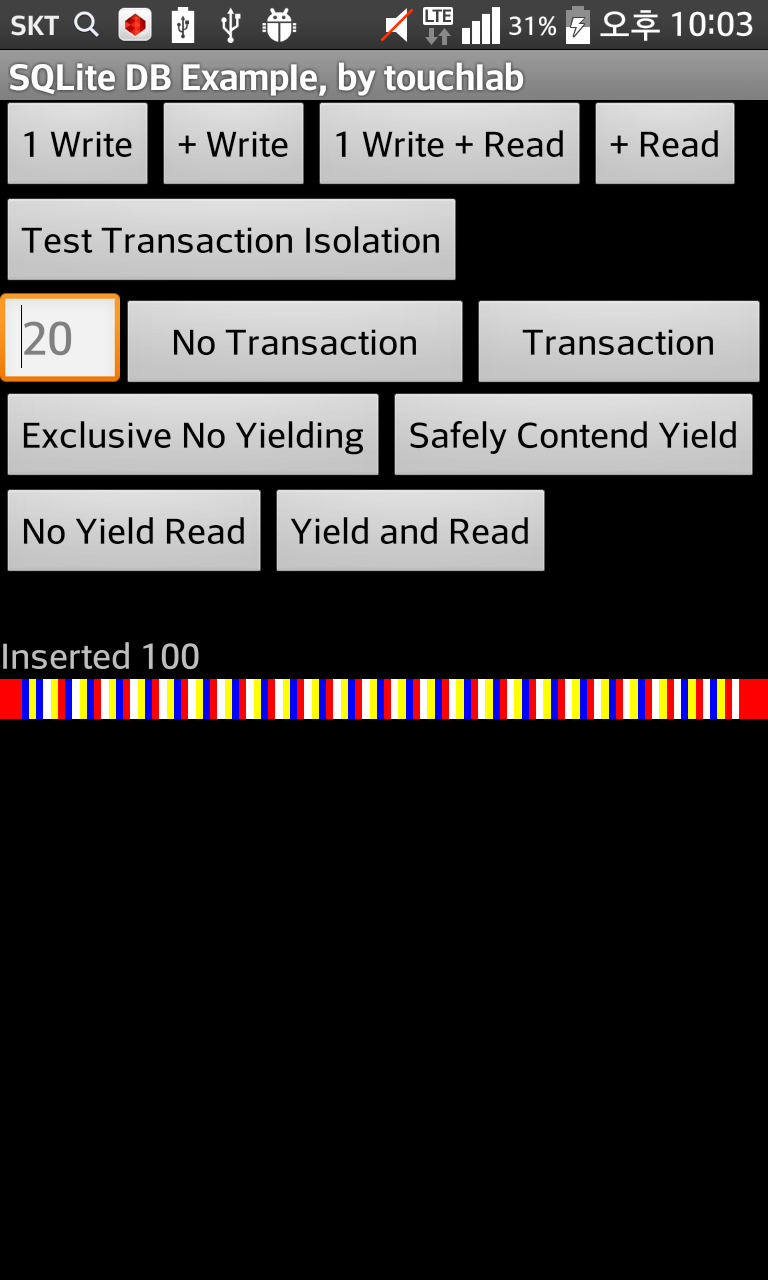
\includegraphics[scale=0.35]{device-sqlite}\\
File IO 성능이 좋지 않던 초기 안드로이드 단말에서는 Lock 문제가 쉽게 드러났지만, 최신 단말에서는 바로 눈에 띄지 않을 수도 있다.\footnote{버전이 높은 것이 항상 나은 것은 아니다. 4.0.4 버전의 특정 단말에서 Lock 에러가 많이 발생한 적도 있다.} 당장 보이지 않는다고 해서 사용자 단말에서도 문제가 없다고 생각하지 말자. QA 테스트에서는 거의 안 나타나던 Lock 에러가 배포 후에 사용자 단말에서는 다량으로 나타난 경우도 있었다.\\

Lock/트랜잭션 관련해서 테스트 샘플 코드는 github에서 찾을 수 있다.
\url{https://github.com/touchlab/Android-Database-Locking-Collisions-Example}
샘플을 테스트한 결과를 얘기해보자.
\begin{enumerate}
\item 여러 스레드에서 1개의 SQLiteDatabase 인스턴스만 가지고 쓰기를 한다. 이때는 Lock 문제가 발생하지 않는다. 

\item 여러 스레드에서 각각 SQLiteDatabase 인스턴스를 가지고 쓰기를 한다. 이때는 Lock 문제가 발생한다. 여러 번 해봐도 문제가 잘 발생하지 않는다면 소스 상에서 스레드 개수를 늘려보자. 계속 늘려가보면 반드시 Lock 문제가 발생한다.

\item 1개의 스레드에서 1개의 SQLiteDatabase 인스턴스를 가지고 계속 쓰기를 하고, 여러 스레드에서 각각 SQLiteDatabase 인스턴스를 가지고서 읽기만 한다면 Lock 문제가 발생한다.

\item 여러 스레드에서 각각 SQLiteDatabase 인스턴스를 가지고서 읽기만 하면 Lock 문제가 발생하지 않는다.

\item 1개의 SQLiteDatabase 인스턴스를 가지고 쓰기 트랜잭션과 읽기를 동시에 실행한다. Lock 문제가 발생하지 않는다.

\item 1개의 SQLiteDatabase 인스턴스를 가지고 쓰기를 하는데 트랜잭션을 쓰지 않는 경우와 쓰는 경우를 비교할 수 있다. 트랜잭션을 쓰는 경우에 시간이 크게 줄어드는 것을 볼 수 있다.

\end{enumerate}

1$\sim$5번의 테스트에서 중요한 것은  SQLiteDatabase 인스턴스를 하나만 가지고 여러 스레드에서 명령을 실행해도 Lock 문제가 발생하지 않는다는 것이다. 이것은 SQLite의 default threading mode가 serialized이기 때문이다. 즉 명령어들은 순차적으로 실행되는 것이다.\footnote{\url{http://stackoverflow.com/questions/11167834/what-is-the-default-threading-mode-of-sqlite-in-android}}\\

threading mode 관련한 내용은 아래 url을 참고하자.\\
\url{http://www.sqlite.org/threadsafe.html}\\

SQLiteDatabase 인스턴스를 1개만 가지고서 serialized mode로 동작한다면 속도가 느려지진 않을까? 결론적으로 그렇다.
쓰기와 읽기가 함께 있는 것이라면 serialized mode가 되어야만 Lock 문제가 없기 때문에 1개의 인스턴스를 사용해야 하지만, 읽기만 있다면 굳이 1개의 인스턴스를 고집할 필요가 없다.

\begin{comment}
\subsubsection{Yield 하기}

\item Exclusive No Yielding과 Safely Contend Yield: SQLiteDatabase에는 yieldContendedSafely라는 메서드가 있어서, 다른 스레드의 명령이 실행되도록 트랜잭션을 끝내는 방법이 있다. 이게 호출될 때까지 성공한 것으로 간주하고 다시 새로운 트랜잭션이 생겨난다. 실행시간이 너무 길다 싶으면 다른 쪽에 양보를 하는 것인데, 전체 실행 속도에는 큰 차이가 보이진 않고, 다른 스레드의 명령이 너무 늦게 실행되는 것을 방지하는 측면에서 사용 가능하다. 이 테스트는 모두 다 쓰기 스레드이다.

\item No Yield Read와 Yield and Read: 쓰기 스레드와 읽기 스레드가 함께 있다. 쓰기 시간이 길어질 때 읽기 쪽에 양보하는 방식이다.
위에서 나온 Yield가 쓰일 만한 곳도 알아보자. 앱이 설치되고 처음 실행될때, 앱에서 사용할 기본 데이터를 위해서\footnote{이를테면 캘린더앱에서는 각 나라의 휴일 정보 같은 것이다. 한 해 것만 가져오는 것이 아니고 1900년부터 100년이 넘는 것을 모두 가져올 수도 있다. 음력이 있는 동양권에서는 더 많은 데이터가 필요하기도 하다.} API를 통해 서버에서 데이터를 가져올 수 있다. 만일 이것이 백만 건이 넘는 데이터라고 하면 JSON  데이터라고 해도 가져오는 데는 큰 부하까지는 걸리지 않을 것이다.\\
이것을 DB에 넣으려고 하면 당연히 Transaction으로 감싸야 한다.
그런데 앱은 처음 화면이 잘 뜨는 것도 중요하다. 
캘린더앱의 경우라면 처음 화면이 뜨고 일정을 조회하려고 DB 쿼리를 실행할 것이다. 그런데 앞에서 백만 건의 넘는 것을 Insert 하느라고 DB를 잡고 있다면, DB 쿼리를 실행할 수 없고 따라서 초기 실행 시간이 체감상 많이 느려질 수 있다.\\ 
그럼 10,000개마다 끊어서 Transaction을 매번 실행할 것인가 하면 그럴 필요가 없다. 바로 SQLiteDatabase.yieldContendedSafely를 10,000개마다 실행해주면 된다.
% 소스 있는 게 좋을 듯 하다. 정말 양보가 되는가?
\end{comment}

% 여기서 WAL을 넣어야 할 듯 하다.
% http://www.sqlite.org/wal.html
% http://sqlite.org/atomiccommit.html

%http://www.sqlite.org/datatype3.html

% http://beets.radbox.org/blog/sqlite-nightmare.html

%http://stackoverflow.com/questions/1005206/does-sqlite-lock-the-database-file-on-reads


%http://gywn.net/2013/08/let-me-intorduce-sqlite/

%http://www.sqlite.org/lockingv3.html
    
\begin{comment}
인덱스 문제가 있거나 테이블 조인 구조가 복잡하다면 쿼리 튜닝이 필요할 수 있다. EXPLAIN PLAN을 쓰는 방법이나 튜닝에 대한 기본 내용들은 인터넷에 많이 찾아 볼 수 있다.\\

09-05 18:47:27.335: E/Database(13396): close() was never explicitly called on database '/data/data/com.nhn.android.alarmclock/databases/alarms.db' 
09-05 18:47:27.335: E/Database(13396): android.database.sqlite.DatabaseObjectNotClosedException: Application did not close the cursor or database object that was opened here
09-05 18:47:27.335: E/Database(13396): 	at android.database.sqlite.SQLiteDatabase.<init>(SQLiteDatabase.java:1847)
09-05 18:47:27.335: E/Database(13396): 	at android.database.sqlite.SQLiteDatabase.openDatabase(SQLiteDatabase.java:820)
09-05 18:47:27.335: E/Database(13396): 	at android.database.sqlite.SQLiteDatabase.openOrCreateDatabase(SQLiteDatabase.java:854)
09-05 18:47:27.335: E/Database(13396): 	at android.database.sqlite.SQLiteDatabase.openOrCreateDatabase(SQLiteDatabase.java:847)
09-05 18:47:27.335: E/Database(13396): 	at android.app.ContextImpl.openOrCreateDatabase(ContextImpl.java:640)
09-05 18:47:27.335: E/Database(13396): 	at android.content.ContextWrapper.openOrCreateDatabase(ContextWrapper.java:203)
09-05 18:47:27.335: E/Database(13396): 	at android.database.sqlite.SQLiteOpenHelper.getWritableDatabase(SQLiteOpenHelper.java:118)
\end{comment}

\subsection{SQLiteOpenHelper}
SQLiteDatabase는 SQLite에 접근하는 클래스로, SQL 명령어를 실행하고 DB를 관리하는 메서드를 가지고 있다. 
SQLite를 사용하기 위해서는 꼭 거쳐야 하는 클래스이지만 실제 앱에서는 SQLiteDatabase를 직접 생성해서 사용하는 경우는 드물다.\footnote{/data/data/[패키지명]/databases가 아닌 다른 위치에 DB를 생성하거나 다른 앱(물론 앱의 공간이 아닌 public한 공간)의 DB를 읽고자 할 때는 SQLiteDatabase를 직접 사용해야 한다.}
바로 Helper 클래스인 SQLiteOpenHelper를 상속해서 사용하는데, SQLiteOpenHelper에서 Database 생성이나 Database 버전 관리를 알아서 해준다.\\

일반적으로 앱은 업데이트됨에 따라, DB에 테이블이 추가되거나 칼럼이 변경되고 앱에 필요한 기본 데이터가 추가되기도 한다. 
그래서 버전 관리는 필수적인데, SQLiteDatabase를 가지고 직접 하지 말고 반드시 SQLiteOpenHelper를 이용하도록 하자.
SQLiteOpenHelper는 추상 클래스이면서 일종의 Template Method 패턴을 만들어 놓은 것으로, 이 클래스를 상속해서 onCreate()와 onUpgrade() 메서드를 구현한 Database Helper를 작성하면 된다.\footnote{허니콤에서 onDowngrade() 메서드도 포함되었지만 이것은 추상 메서드는 아니어서 구현이 필수는 아니다.}\\

아래 코드는 ApiDemos에 있는 Database Helper를 조금 수정한 것이다.
\begin{lstlisting}[frame=single] 
public class DatabaseHelper extends SQLiteOpenHelper {

	private static final String DATABASE_NAME = "loader_throttle.db";
	private static final int DATABASE_VERSION = 2;

	DatabaseHelper(Context context) {
		super(context, DATABASE_NAME, null, DATABASE_VERSION); // (1)
	}

	@Override
	public void onCreate(SQLiteDatabase db) {
		db.execSQL("CREATE TABLE " + MainTable.TABLE_NAME + " ("
				+ MainTable._ID + " INTEGER PRIMARY KEY,"
				+ MainTable.COLUMN_NAME_DATA + " TEXT" + ");");
		...
	}

	@Override
	public void onUpgrade(SQLiteDatabase db, int oldVersion, int newVersion) {
		for (int i = oldVersion + 1; i <= newVersion; i++) { // (2)
			 processUpgrade(db, i);
		}
	}
}
\end{lstlisting}
여기서 살펴볼 게 몇 가지 있다.
\begin{itemize}
\item 7라인(1)의 생성자에 DATABASE\_NAME이 들어가는 것이 바로 DB 파일명이다.
그럼 DB를 여러 개 쓴다면 Database Helper도 여러 개 필요하다는 말일까? 그렇다. 
하나의 앱에서 필요에 의해서 여러 DB를 사용할 수도 있고, 이때 기본적으로 Database Helper가 각각 필요하다.
가능하면 DB를 하나로 사용하는 것이 좋지만, 상황상 어쩔 수 없는 케이스도 있고 DB Lock 문제를 효과적으로 대응하기 위해서 DB를 분리할 수도 있다(읽기 전용 데이터를 위한 DB, 읽기+쓰기 용도 DB).\\

테이블이 동일하고 데이터 구조가 다른 게 없다면 그때는 어떡할까? 
이를테면 로그인 기반의 앱이라면, 공통으로 사용하는 데이터를 위한 공통 DB가 있고 각 사용자별 DB가 있을 수 있다. 
각 사용자별 DB는 당연히 동일한 테이블 구조를 갖고 있다. 이때는 DB 파일명을 상수를 만들지 않고 동적으로 전달하면 된다.
\begin{lstlisting}[frame=single] 
    DatabaseHelper(Context context) {
        super(context, getAuth().getLoginId() + ".db", null, DATABASE_VERSION);
    }
\end{lstlisting}

\item 생성자의 세 번째 파라미터는 거의 null을 넣는다. 
쿼리 결과로 Cursor 구현체인 SQLiteCursor를 쓰지 않는다면, Cursor 구현을 생성하는 Factory인 
SQLiteDatabase.CursorFactory를 새로 만들어서 파라미터에 전달할 수 있지만 필요한 경우가 사실상 없다.
%쿼리 결과로 SQLiteCursor를 쓰지 않는 경우라면, Cursor를 생성하는 SQLiteDatabase.CursorFactory를 새로 만들어서 넣는 게 가능하지만, 필요한 경우가 사실상 없다.

\item DB 생성은 어느 시점에 될까? SQLiteOpenHelper 생성자에서 하는 것으로 생각할 수 있지만 그렇지 않다.
실제로 DB 열기/생성(openOrCreate)은 SQLiteOpenHelper의 getReadableDatabase()나 getWritableDatabase() 메서드를 호출할 때이다.
더 정확하게 얘기하면 SQLiteOpenHelper에는 SQLiteDatabase 인스턴스를 1개 가지고 있는데 이 인스턴스가 앞에 이미 생성되었으면 그것을 사용하고, 그렇지 않은 경우에 생성하고서 onCreate()나 onUpgrade() 메서드가 실행된다.

\item DB 테이블 변경 시에는 Database Helper 생성자에 새로운 버전을 전달하고, 
SQLiteOpenHelper의 onUpgrade(SQLiteDtabase db, int oldVersion, int newVersion) 메서드에 변경 내용을 적용하면 된다. 
이때 일반 패턴은 20라인(2)과 같이 for 문을 사용해서 oldVersion과 newVersion 범위 사이에 DB 버전에 했던 작업들을 처리하는 것이다.

\item onCreate() 메서드에는 최신 DB 스키마와 데이터를 반영해야 한다. 
onCreate() 메서드는 앱이 처음 DB를 생성할 때 호출된다. DB 버전이 1, 2, 3, 4 이렇게 바뀌면서 스키마와 데이터가 변경되었다고 하자. 
버전이 1일 때 앱이 DB를 생성한다면 onCreate() 메서드가 호출되고, 중간에 앱을 업데이트하지 않다가 최신 버전으로 업데이트했다면 onUpgrade() 메서드가 호출된다.
그럼 버전이 4일때 처음 앱을 설치한다면 어떨까? 바로 onCreate() 메서드만 호출되고 onUpgrade() 메서드는 호출되지 않는다. 
개발하다 보면 onCreate()와 onUpgrade()가 순차적으로 호출되는 것으로 가끔 착각하게 되어서 언급하였다. onCreate()와 onUpgrade()는 둘 중에 하나만 호출된다.

\item DB 버전 업그레이드가 필요할 때 빠뜨려서는 안 된다. 예를 들어, 테이블 설계에 문제 있는 버전이 배포되었다고 하자.
마음 같아서는 다시 작성해서 동일한 버전으로 하면 코드도 깔끔할 것 같은데, 기존에 이 버전을 사용중인 단말은 DB 버전이 동일하므로 onUpgrade()는 실행되지 않고 변경된 테이블을 사용할 수 없다.
버전을 올리고서 onUpgrade()에서 테이블 구조를 변경하는 코드가 들어가는 게 정상적인 방법이다.

\item onCreate()와 onUpgrade() 메서드에서 하는 작업은 테이블 생성/수정 뿐 아니라 많은 기본 데이터 INSERT 등도 필요하다. 
예를 들어, INSERT는 건당 시간이 얼마 안 걸리지만 1,000건, 10,000건이 된다면 속도가 대폭 떨어질 것을 예상할 수 있다.
그래서 트랜잭션을 쓰려고 하는데 SQLiteOpenHelper에는 이미 onCreate()와 onUpgrade() 메서드를 트랜잭션으로 감쌌기 때문에 또 다시 트랜잭션을 고려할 필요가 없다.\footnote{SQLiteOpenHelper가 Template Method로서 의미 있는 부분이다.}

\item DATABASE\_NAME 위치에 null을 넣으면 파일 DB가 아닌 메모리 DB가 된다. 파일 DB라도 속도가 느리진 않지만 메모리 DB는 그보다 훨씬 속도가 빠르다. 
DB가 닫히면 함께 사라져버리는 휘발성 DB이므로 일종의 캐시 용도로 사용하는 것이 좋다.
코드 상에서 캐시 자료구조를 만들어도 되는데, 굳이 메모리 DB를 쓰면 좋은 케이스는 무엇일까? 바로 그 안에서 쿼리를 실행할 수 있다는 점이다.
예를 들어, 여러 칼럼이 있고 각 칼럼별로 정렬을 바꾸어주는 기능이 있다면, 정렬할 때마다 File IO를 하는 것보다는 메모리 DB에 담아놓고서 쿼리로 정렬하면 결과가 훨씬 빨라진다. 
파일 DB에서 원시(raw) 데이터를 가져와서 조합해서 생성한 결과 목록을 메모리 DB에 저장해서 사용하는 것도 고려해 볼 수 있다.\\

당연한 얘기지만 메모리 DB에서는 DB 버전 업그레이드가 의미가 없으므로 version은 신경쓸 필요가 없다. 1로 놓고 다시는 변경하지 말자.

\item Database Helper는 앱 전체에 걸쳐 단일 인스턴스를 가지고 있어야 DB Lock 문제에서 자유롭다. 
그래서 일반적으로 아래와 같이 싱글톤 패턴을 만들어서 사용한다. 싱글톤 패턴에 대해서 11장에서 다시 설명하기로 한다.
\begin{lstlisting}[frame=single] 
public static DatabaseHelper extends SQLiteOpenHelper  {
   private static DatabaseHelper instance;
 
  public static synchronized DatabaseHelper getInstance(Context context) {
     if (instance == null) {
        instance = new DatabaseHelper(context.getApplicationContext()); // (1)
     }
    return instance;
   }
 
   private DatabaseHelper(Context context) {
       ...
   }
}
\end{lstlisting}
6라인(1)에서 context가 아닌 context.getApplicationContext()를 전달한 것을 주목하자.
생성자가 private으로 감추어져 있으므로 사용하는 쪽에서는 getInstance()로 가져와서 사용한다.
\begin{lstlisting}[frame=single] 
DatabaseHelper dbHelper = DatabaseHelper.getInstance(context);
\end{lstlisting}

\item close() 메서드는 실제 호출할 일이 거의 없다.
SQLiteOpenHelper의 close()는 SQLiteDatabase 인스턴스의 close()를 호출하고, SQLiteDatabase 인스턴스를 null로 만든다. 
매번 close()를 호출하지 않고서 SQLiteDatabase 인스턴스를 계속 재사용해도 문제가 없고, 또 다른 이유는 close() 실행 시점 때문에 문제가 발생할 수 있다는 것이다.\\

A 스레드에서 getWritableDatabase() 이후에 쿼리를 실행한다고 하자. B 스레드에서는 뭔가 작업을 하고 close()를 실행한다. 시점에 따라서 A 스레드에서 getWritableDatabase() 이후에 B 스레드에서 close()가 실행되고, 이것을 가지고 A 스레드에서 쿼리한다면  NullPointerException이 발생하게 된다. 
%  에러 메시지 보여주자
\item onConfigure(SQLiteDatabase db) 메서드와 onOpen(SQLiteDatabase db) 메서드가 있다. onConfigure() 메서드는 SQLiteDatabase 생성/열기 이후, onCreate()와 onUpgrade() 메서드 전에 실행되는 것으로 write-ahead logging이나 foreign key support 같은 기능을 활성화하는 작업 등을 할 수 있다. onOpen() 메서드는 onCreate()와 onUpgrade() 이후에 database connection 설정을 변경할 때 사용한다.

\end{itemize}

\section{ContentProvider}
ContentProvider는 여러 앱 간에 데이터를 공유할 필요가 있을 때 사용한다. 데이터 소스는 굳이 DB일 필요는 없다. 
파일이든 네트워크를 통해서 구하는 값이든 다 데이터 소스로 가능하다. 다만 API가 DB를 데이터 소스로 사용하는 것에 더 맞게 디자인되어 있다.\\

ContentProvider 접근은 ContentResolver를 통해서만 가능하다. 그리고 Context의 getContentResolver() 메서드를 통해서만 ContextResolver를 구할 수 있다.  
% 그림 필요
ContextResolver는 일종의 Proxy인데, 해당하는 Uri의 ContentProvider를 찾는 역할을 한다.
% 퍼미션 체크는 ContentProvider에서 한다.
ContentResolver는 추상 클래스이고 실제 사용하는 클래스는 ContextImpl의 내부 클래스인 ApplicationContentResolver이다.

\subsection{ContentProvider 적용}
개발자 가이드에 의하면 로컬 프로세스에서만 사용하려면 ContentProvider를 사용하지 않는 것이 권장된다. 
ContentResolver를 거치는 것보다 직접 DB를 접근하는 것이 속도가 훨씬 빠르다.\\

한 앱에서도 ContentProvider를 쓰면 유용한 경우를 들어보자(이 때문에 어떤 문서에서는 가능하면 DB 관련 코드는 ContentProvider를 쓰라고 하기도 한다).
\begin{itemize}
\item 메서드 시그너처를 따라야 하므로 API 일관성을 유지할 수 있다.
\item CursorLoader, AsyncQueryHandler와 같은 유용한 클래스들이 ContentProvider의 Uri가 전달되어야만 동작한다.
\item 한 앱에서도 프로세스가 분리될 수 있다. 이를테면 Service가 메모리 사용이 많아서 프로세스를 분리하고 각 프로세스에서 Database Helper를 사용한다면, 싱글톤이 유지되지 않아서 Lock 문제가 언제든 발생할 수 있다.
이때 앱 프로세스에 ContentProvider를 두고, 이 ContentProvider를 Service 프로세스에서 ContentResolver를 통해서 접근하면 유일한 Database Helper를 유지할 수 있다. %이미지 추가?
\end {itemize}

그럼 로컬 프로세스에서 ContentProvider를 쓰는 단점은 무엇일까?
\begin{itemize}
\item 직접 DB에 접근하는 것에 비해서 속도가 조금 느리다.
\item groupBy, having, limit 같은 파라미터를 ContentResolver의 메서드에 전달할 수 없다. 
필요한 경우 Uri나 쿼리 파라미터에 억지로 끼워넣어서 전달해야 한다. 
\item ContentResolver를 통하므로 별도의 public 메서드를 만들어도 접근할 수 없다.
\end {itemize}

가이드가 혼재되어 있는데 결론을 내려보자.
로컬 프로세스에서는 ContentProvider를 쓰지 않는 것을 먼저 고려하자. ContentProvider를 사용하는 장점이 꼭 필요하다면, 그때 ContentProvider를 쓰기로 하자.
다만 직접 DB에 접근하는 코드에서도 메서드 시그너처를 ContentProvider와 유사하게 만들면, 이후에 변경이 수월할 수 있다.
프로세스가 분리되거나 다른 앱에서 DB 접근이 필요하다면, 필요한 부분만 ContentProvider로 접근해서 DB Access(내부용) + ContentProvider(외부용)으로 하는 것도 가능한 방법이다.\\

%https://thenewcircle.com/s/post/1375/android_content_provider_tutorial

코드 \ref{src:provider}은 안드로이드 샘플 프로젝트인 NotePad에서 ContentProvider를 만든 예이다. 
ContentProvider는 다른 컴포넌트와는 달리 만드는 방법이 정형화되어 있다. 
ContentResolver를 통해서만 접근하기 때문에 별도의 public 메서드는 의미가 없다.

\begin{lstlisting}[frame=single, caption=ContentProvider 예, label=src:provider] 
public class NotePadProvider extends ContentProvider {
	private static final String TAG = "NotePadProvider";

	private static final String DATABASE_NAME = "note_pad.db";
	private static final int DATABASE_VERSION = 2;

	...

	private static final UriMatcher sUriMatcher;

	private DatabaseHelper mOpenHelper;

	static {
		sUriMatcher = new UriMatcher(UriMatcher.NO_MATCH);
		sUriMatcher.addURI(NotePad.AUTHORITY, "notes", NOTES);
		sUriMatcher.addURI(NotePad.AUTHORITY, "notes/#", NOTE_ID);
		...
	}

	static class DatabaseHelper extends SQLiteOpenHelper {

		DatabaseHelper(Context context) {
			super(context, DATABASE_NAME, null, DATABASE_VERSION);
		}

		@Override
		public void onCreate(SQLiteDatabase db) {
			db.execSQL("CREATE TABLE " + NotePad.Notes.TABLE_NAME + " ("
					+ NotePad.Notes._ID + " INTEGER PRIMARY KEY,"
					+ NotePad.Notes.COLUMN_NAME_TITLE + " TEXT,"
					+ NotePad.Notes.COLUMN_NAME_NOTE + " TEXT,"
					+ NotePad.Notes.COLUMN_NAME_CREATE_DATE + " INTEGER,"
					+ NotePad.Notes.COLUMN_NAME_MODIFICATION_DATE + " INTEGER"
					+ ");");
		}

		@Override
		public void onUpgrade(SQLiteDatabase db, int oldVersion, int newVersion) {
			...
		}
	}

	@Override
	public boolean onCreate() {
		mOpenHelper = new DatabaseHelper(getContext()); // (1)
		return true;
	}

	@Override
	public Cursor query(Uri uri, String[] projection, String selection,
			String[] selectionArgs, String sortOrder) {
		...
		SQLiteDatabase db = mOpenHelper.getReadableDatabase();

		Cursor c = qb.query(db, // The database to query
				projection, // The columns to return from the query
				selection, // The columns for the where clause
				selectionArgs, // The values for the where clause
				null, // don't group the rows
				null, // don't filter by row groups
				orderBy // The sort order
				);

		c.setNotificationUri(getContext().getContentResolver(), uri);
		return c;
	}

	@Override
	public String getType(Uri uri) {
		switch (sUriMatcher.match(uri)) {
		case NOTES:
			return NotePad.Notes.CONTENT_TYPE;
		case NOTE_ID:
			return NotePad.Notes.CONTENT_ITEM_TYPE;
		default:
			throw new IllegalArgumentException("Unknown URI " + uri);
		}
	}

	@Override
	public Uri insert(Uri uri, ContentValues initialValues) {
		...
		SQLiteDatabase db = mOpenHelper.getWritableDatabase();
		long rowId = db.insert(NotePad.Notes.TABLE_NAME,
				NotePad.Notes.COLUMN_NAME_NOTE, 
				values 
				);

		if (rowId > 0) {
			Uri noteUri = ContentUris.withAppendedId(
					NotePad.Notes.CONTENT_ID_URI_BASE, rowId);
			getContext().getContentResolver().notifyChange(noteUri, null);
			return noteUri;
		}
		throw new SQLException("Failed to insert row into " + uri);
	}

	@Override
	public int delete(Uri uri, String where, String[] whereArgs) {
		SQLiteDatabase db = mOpenHelper.getWritableDatabase();
		...
		count = db.delete(NotePad.Notes.TABLE_NAME, // The database table name
					finalWhere, // The final WHERE clause
					whereArgs // The incoming where clause values.
					);

		..
		getContext().getContentResolver().notifyChange(uri, null);
		return count;
	}

	@Override
	public int update(Uri uri, ContentValues values, String where,
			String[] whereArgs) {
		SQLiteDatabase db = mOpenHelper.getWritableDatabase();
		...
		count = db.update(NotePad.Notes.TABLE_NAME, 
					values, 
					where, 
					whereArgs 
					);
		...
		getContext().getContentResolver().notifyChange(uri, null);
		return count;
	}

}
\end{lstlisting}
\begin{itemize}
\item ContentProvider를 사용하면 멀티 스레드 환경에서 Lock 문제가 없이 잘 동작하기 때문에 ContentProvider에서 Lock을 제어한다고 오해하는 경우가 있다. 
Lock 문제가 발생하지 않는 것은 ContentProvider를 써서 그런 것이 아니라 ContentProvider를 만드는 일반적인 패턴으로 인한 것이다.
45라인(1)을 보면 onCreate() 메서드에서 Database Helper를 하나 생성해놓고 이것을 사용하고 있다.
onCreate()는 처음 ContentProvider를 사용할 때 단 한번만 실행되고, ContentProvider는 단말에서 오직 하나만 존재하기 때문에 Database Helper도 오직 하나뿐이다. 따라서 내부적으로 명령어가 serialization되면서 Lock 문제가 없는 것이다.

\item ContentProvider의 onCreate() 메서드는 Application의 onCreate() 메서드 이전에 실행된다.\footnote{ActivityThread의 handleBindApplication() 메서드를 분석해보자.}
따라서 Application의 onCreate() 메서드가 먼저 실행된다고 가정하면 안된다.
복잡한 앱에서는 Application의 onCreate() 메서드에서 앱 전체적으로 사용하는 인스턴스를 미리 생성하는 역할을 하기도 한다. ContentProvider에서도 Application에서 생성한 것을 쓰고 싶지만 순서를 주의하도록 하자.
ContentProvider의 onCreate()는 메인 스레드에서 실행하고 다른 메서드는 일반적으로 별도 스레드에서 실행하므로(로컬에서도 ContentProvider는 스레드에서 호출하도록 권장되고, Binder를 통한 외부 앱의 접근은 Binder 스레드를 거쳐 실행), ContentProvider의 메서드 간에는 스레드 안정성에 주의하도록 하자. 멤버 변수를 함부로 쓰면 안된다는 얘기이다.

\item insert/update/delete 메서드에서 DB 명령 실행 후에 getContext().getContentResolver().not\-ifyChange\-(uri, null)를 호출한다. ContentResolver에는 registerContentObserver() 메서드가 있어서 데이터가 변경되면 알 수 있도록 ContentObserver를 등록하는데, 이 ContentObserver에 알림을 주기 위한 것이다. 
ContentObserver에는 어떤 데이터가 변경되었는지 알리지는 않고 변경되었는지 여부만 전달한다. 
그러면 무슨 쓸모가 있는가 의문이 생기는데,
query() 메서드에서 리턴 결과인 Cursor에는 requery()라는 메서드가 있어서 새로 조회할 수 있다. 특히 CursorAdaper는 내부에 ContentObserver가 등록되어 있어서 notifyChange()를 받으면 requery()를 실행한다.

\end{itemize}
% ContentProvider call 메서드도 있다.(이것이 안드로이드다 참고)

\subsection{배치 실행}
% http://surprisen.egloos.com/2504139
ContentProvider에서는 여러 명령어를 한꺼번에 실행할 수 있는 applyBatch() 메서드를  제공한다. 
applyBatch() 메서드를 보면 속도 향상을 위해서 트랜잭션을 쓰는 것으로 혼동할 수도 있지만, 실제로 하는 일은 ContentProviderOperation 목록을 한꺼번에 전송해놓고 순차 실행하는 것에 지나지 않는다. 
\begin{lstlisting}[frame=single] 
ArrayList<ContentProviderOperation> operations 
	= new ArrayList<ContentProviderOperation>();
operations.add(ContentProviderOperation.newInsert(NotePad.CONTENT_URI) // (1)
	.withValue(NotePad.Notes.COLUMN_NAME_TITLE, "Lunch")
	.withValue(NotePad.Notes.COLUMN_NAME_NOTE, "Kimchi")
	.withValue(NotePad.COLUMN_NAME_CREATE_DATE, 
		Long.valueOf(System.currentTimeMillis()))
	.build());
operations.add(ContentProviderOperation.newUpdate(NotePad.CONTENT_URI) // (2)
	.withSelection(NotePad.Notes._ID + "=?", new String[] {3})
	.withValue(NotePad.Notes.COLUMN_NAME_TITLE, "Lunch2")
	.withValue(NotePad.Notes.COLUMN_NAME_NOTE, "Kimchi2")
	.withValue(NotePad.Notes.COLUMN_NAME_MODIFICATION_DATE, 
		Long.valueOf(System.currentTimeMillis()))
	.build());
operations.add(ContentProviderOperation.newDelete(Memos.CONTENT_URI) // (3)
	.withSelection(NotePad.Notes._ID + "=?", new String[] {5})
	.build());

mContext.getContentResolver().applyBatch(NotePad.AUTHORITY, operations); // (4)
\end{lstlisting}
\begin{itemize}
\item 3라인(1), 9라인(2), 16라인(3)에서 ContentProviderOperation(Insert/Update/Delete용)을 ArrayList에 추가한다. 
newInsert/newUpdate/newDelete 같은 메서드는 Builder 패턴을 사용해서 ContentProviderOperation 인스턴스를 만들어 낸다.
\item 20라인(4)에서 applyBatch() 메소드를 통해 ArrayList에 쌓아둔 작업들을 한꺼번에 보낸다.
\end{itemize}

다른 프로세스에서 실행한다면 Binder를 거쳐야 하는데, 하나씩 명령어를 주고받는 것보다 한꺼번에 보내는 것으로 속도 향상은 있지만 트랜잭션을 쓰는 것처럼 속도 향상이 큰 것은 아니다.
트랜잭션을 써서 속도를 향상시키고 싶다면,
ContentProvider에서 applyBatch(ArrayList$<$ContentProviderOper\-ation$>$ operations) 메서드를 오버라이드하는 방법이 있다.
\begin{lstlisting}[frame=single] 
@Override
public ContentProviderResult[] applyBatch(
		ArrayList<ContentProviderOperation> operations) {
	SQLiteDatabase db = mOpenHelper.getWritableDatabase();
	db.beginTransaction();
	try {
     	ContentProviderResult[] result = super.applyBatch(operations);
     	db.setTransactionSuccessful();
     	return result;
   	} finally {
     	db.endTransaction();
   	}
}
\end{lstlisting}
트랜잭션으로 감싸는 코드를 applyBatch() 메서드에 적용하였다.

\begin{comment}
\begin{lstlisting}[frame=single] 
07-08 10:13:30.923: E/SQLiteOpenHelper(25079): android.database.sqlite.SQLiteDatabaseLockedException: database is locked (code 5): , while compiling: PRAGMA journal_mode
07-08 10:13:30.923: E/SQLiteOpenHelper(25079): 	at android.database.sqlite.SQLiteConnection.nativePrepareStatement(Native Method)
\end{lstlisting}

SQLiteQueryBuilder.buildQueryString 이것으로 쿼리문 결과 볼 수 있다.

bulk insert update
http://www.mysamplecode.com/2011/10/android-sqlite-bulk-insert-update.html

I/O 발생으로 가능하면, AsyncTask 나 별도 Thread에서 실행하는 것을 권장한다.
API 11에서부터 CursorLoader를 사용할 수 있는데, AsyncTask를 사용해서, Content Provider를 통해서 값을 가져온다.

LIKE 구문은 신경을 쓰자..
http://www.mail-archive.com/sqlite-users@sqlite.org/msg14482.html

필요한 경우 index를 생성한다.


% http://androcat.egloos.com/1778615
% http://developer.android.com/training/notepad/notepad-ex3.html
% http://stackoverflow.com/questions/4940308/im-getting-a-database-object-not-closed-exception-in-sqlite-android-but-im
 

%http://www.enterra-inc.com/techzone/handling_sql_issues/

remote에서 contentProvider를 호출할 경우 CursorWindow를 복사해버린다. multiprocess는 확인해봐야 한다.


Conent Provider를 사용하지 않을 때에는 칼럼명을 굳이 상수화 하지 않도록 한다.

%http://stackoverflow.com/questions/2647542/android-threading-and-database-locking
%http://www.androiddesignpatterns.com/2012/05/correctly-managing-your-sqlite-database.html
%http://charlie0301.blogspot.kr/2013/07/sqlite-and-android-sqlite.html

content prefix는 content provider에 의해 데이타가 제공된다는 의미이다.

content://com.example.transportationprovider/trains

ContentProvider의 insert 메서드는 리턴이 Uri로 받은 값을 가지고 입력한 id를 얻을 수 있다.
\begin{verbatim}
long rowId = database.insert(values);

		if (rowId > 0) {

			Uri memoUri = ContentUris.withAppendedId(CONTENT_URI, rowId);

      getContext().getContentResolver().notifyChange(memoUri, null);

			return memoUri;

		}

=>

			String id = uri.getPathSegments().get(1);
\end{verbatim}



액티비티에서는  managedQuery  메서드를 바로 사용하면 된다.
insert, update, delete는 getContentResolver() 하고서 메서드를 호출한다.
\end{comment}

\section{SQLite/ContentProvider 관련 팁}
\subsection{쿼리 실행 확인}
일반적으로 쿼리 속도를 체크하기 위해서 코드 상에 쿼리 실행 전후 시간 차이를 로그로 남겨서 확인한다.
이 방식도 지속적으로 확인이 필요할 때는 유용하지만, 그 시기가 지나면 불필요한 로깅 코드가 남게 된다.
단순하게 실행 속도를 체크하는 방법을 보자.\\

adb shell에서 dumpsys dbinfo를 하면 DB 별로 최근 쿼리 실행 속도와 바인드된 파라미터들(bindArgs)을 확인할 수 있다(단말에서는 보안상 bindArgs가 잘 나오지 않는다).
가장 최근 것부터 나오므로 순서상 밑의 것부터 보면 된다(쿼리를 prepare하고 execute하는 것을 볼 수 있다).

\begin{lstlisting}[frame=single] 
** Database info for pid 1008 [system] **

Connection pool for /data/data/com.android.providers.settings/databases/settings.db:
  Open: true
  Max connections: 4
  Available primary connection:
    Connection #0:
      isPrimaryConnection: true
      onlyAllowReadOnlyOperations: false
      Most recently executed operations:
        0: [2014-09-30 10:40:04.548] executeForLastInsertedRowId took 5ms 
        	- succeeded, sql="INSERT INTO system(value,name) VALUES (?,?)", 
			bindArgs=["1", "volume_ring_last_audible_speaker"]
        1: [2014-09-30 10:40:04.548] prepare took 0ms - succeeded, 
        	sql="INSERT INTO system(value,name) VALUES (?,?)"
	...
  Available non-primary connections:
    Connection #1:
      isPrimaryConnection: false
      onlyAllowReadOnlyOperations: true
      Most recently executed operations:
        0: [2014-09-30 11:32:32.135] executeForCursorWindow took 0ms 
        	- succeeded, sql="SELECT _id, name, value FROM secure"
        1: [2014-09-30 11:32:32.135] prepare took 0ms - succeeded, 
        	sql="SELECT _id, name, value FROM secure"
	...
  Acquired connections:
    <none>
  Connection waiters:
    <none>
\end{lstlisting}
dumpsys dbinfo 명령어도 모든 앱의 DB 히스토리를 모두 출력하기 때문에 내용이 많다. dbinfo에 쓸 수 있는 옵션은 pid가 있다. 
만일 com.suribada.myhome 패키지의 DB 쿼리 내용을 알고 싶다면 ps | grep com.suribada.myhome으로 pid를 알아낸 다음에 dumpsys dbinfo 1004 와 같이 실행하면 된다.\\

dumpsys dbinfo 명령어는 속도 체크 뿐 아니라 쿼리가 원하는 시점에 실행되는지 체크하는데도 쓰일 수 있다.
여러 스레드에서 쿼리를 실행한다면, 일상적으로 문제가 없다가도 특정한 조건에서 가장 필요로 하는 쿼리가 곧바로 실행되지 않을 수 있다.\\

예를 들어, 화면이 처음 실행될 때에 내부적으로 서버와 데이터 동기화가 실행되면서 화면에도 데이터를 조회해서 보여줘야 한다. 
동기화 중에는 트랜잭션 구간이 있는데 동기화할 데이터가 많고 이런 트랜잭션이 먼저 실행된다면, 조회 쿼리는 그 이후로 미뤄지고 만다. 
동기화할 데이터가 많은 상태까지 테스트하지 못해서, 이런 케이스는 개발 중에는 잘 모를 수도 있다.\\

관련해서 샘플을 만들어보자.
\begin{lstlisting}[frame=single] 
	private DictionaryOpenHelper dbHelper;

	@Override
	protected void onCreate(Bundle savedInstanceState) {
		super.onCreate(savedInstanceState);
		...
		dbHelper = DictionaryOpenHelper.getInstance(this); // (1)
	}

	public void onClickButton1(View view) {
		new Thread(new Runnable() { // (2)

			@Override
			public void run() {
				Log.d("suribada", "Thread1 start");
				SQLiteDatabase db = dbHelper.getReadableDatabase();
				Cursor cursor = db.query(WordTable.TABLE_NAME, 
					null, null, null, null, null, WordTable.COLUMN_KEYWORD); // (3)
				Log.d("suribada", "cursor.count=" + cursor.getCount());
				cursor.close();
			}

		}).start();
		
		new Thread(new Runnable() { // (4)

			@Override
			public void run() {
				Log.d("suribada", "Thread2 start");
				SQLiteDatabase db = dbHelper.getWritableDatabase();
				Random random = new Random();
				db.beginTransaction(); // (5)
				try {
					for (int i = 0; i < 10; i++) {
						int num = random.nextInt(1024);

						ContentValues values = new ContentValues();
						values.put(WordTable.COLUMN_KEYWORD, "apple" + num);
						values.put(WordTable.COLUMN_DEFINITION, 
							"a round fruit " + num);
						values.put(WordTable.COLUMN_PRONUNCIATION, "aepl " + num);
						values.put(WordTable.COLUMN_LAST_UPDATE_TIME,
							System.currentTimeMillis());
						db.insert(WordTable.TABLE_NAME, null, values);
						SystemClock.sleep(1000); // (6)
					}
					db.setTransactionSuccessful();
				} finally {
					db.endTransaction();  // (7)
				}
			}

		}).start();
	}
\end{lstlisting}	
\begin{itemize}
\item 7라인(1)에서 여러 스레드에서 공통으로 사용할 dbHelper 변수를 생성하였다. DB Lock 문제가 발생하지 않으려면 하나의 dbHelper를 사용해야 한다.
\item 11라인(2)과 25라인(4)에서 2개의 스레드를 시작한다.
11라인의 스레드는 단순 조회이다.
25라인의 스레드는 데이터를 10개 입력하는데 45라인(6)에서 1초간 sleep하기 때문에(시간이 걸리는 것을 시뮬레이션) 최소 실행 시간은 10초이다. 32라인(5)에서 트랜잭션을 시작하고 49라인(7)에서 트랜잭션을 종료한다.
\item 스케줄링에 의해서 첫 번째 스레드가 운 좋게 먼저 실행된다면 다행이지만, 두 번째 스레드의 32라인(5)에서 beginTransaction() 메서드가, 첫 번째 스레드의 17라인(3)에서 query() 메서드보다 먼저 실행된다면 어떤 일이 발생할까? 바로 명령어가 serialization되기 때문에 두 번째 스레드의 49라인(startTransaction $\sim$ endTransaction)까지 첫 번째 스레드의 18라인이 대기한다. 사용자 입장에서는 단순 조회라서 금방 되어야 하는데 10초 이상이 걸리는 것이다. 
\end{itemize}

이 상황은 앞서 얘기한 동기화를 하느라고 조회 쿼리가 늦어지는 것과 동일한 케이스이다. 
서버와 데이터를 동기화하는 앱에서 많이 쓰이는 패턴은 아래와 같다.
\begin{enumerate}
\item startService()를 실행하여 Service의 백그라운드 스레드에서 서버 데이터를 가져와 DB에 반영한다. 이때 속도 향상을 위해서 트랜잭션을 사용한다(시간이 얼마나 걸릴지 알 수 없다. 사용자 데이터는 천차만별이다).
\item 첫 화면은 AsyncTask를 이용해서 기존 DB의 데이터를 조회해서 UI에 반영한다. 
\item 동기화가 완료되면 DB에 다 반영되었으므로 Service에서 sendBroadcast()를 실행하고 화면에서는 AsyncTask로 변경된 결과를 다시 조회한다.
\end{enumerate}

1번 때문에 2번이 늦어지는 상황이 이해될 것이다. 원리를 모른다면 ``도대체 왜 그럴까?''하면서 해결할 수 없는 문제가 된다. 
필자의 경우에도 이 문제를 처음 겪었을 때 원인을 미처 생각하지 못했던 기억이 있다. 
그럼 이 문제는 어떻게 해결해야 할까? 바로 2번 작업이 최초 한번은 실행되고 난 다음에 startService()를 실행하는 것이다. 
단지 순서를 바꾸기만 하면 되는 것이다.\\

원하는 시점에 쿼리가 실행되지 않는 원인으로, 사용하는 라이브러리의 쿼리 문제 가능성도 생각할 수 있다. 이를테면 전체 공휴일 정보를 제공하는 라이브러리에서 DB로 정보를 제공할 수도 있다.
문제 상황이 발생했을 때 dumpsys를 통해 확인해보고, 실행 시점을 조정하거나 라이브러리를 재검토해보자.

\subsection{ContentProvider 예외 확인}
외부 프로세스에서 ContentProvider에 접근할 때 ContentProvider를 제공하는 쪽에서 문제가 발생하면, 예외 스택이 그대로 외부 프로세스에 전달되지 않는다.
아래처럼 NullPointerException이 발생했지만, 왜 발생했는지 더 이상 스택이 보이지 않는 걸 볼 수 있다.
\begin{lstlisting}[frame=single] 
Caused by: java.lang.NullPointerException 
	at android.os.Parcel.readException(Parcel.java:1471) 
at android.database.DatabaseUtils.readExceptionFromParcel(DatabaseUtils.java:185) 
at android.database.DatabaseUtils.readExceptionFromParcel(DatabaseUtils.java:137) 
at android.content.ContentProviderProxy.query(ContentProviderNative.java:413) 
at android.content.ContentResolver.query(ContentResolver.java:464) 
at android.content.ContentResolver.query(ContentResolver.java:407
...
\end{lstlisting}
DB가 데이터 소스인 경우는 별로 그럴 일이 없지만, 네트워크나 파일, 또는 로직을 통해 생성한 결과 등을 데이터 소스로 사용한다면 이런 예외 케이스는 원인을 확인해야 한다.\\

그럼 ContentProvider를 제공하는 쪽에서는 크래시가 발생하는가 하면 그렇지 않다. 바로 Exception을 잡아서 Binder로 전달하는 값에 숫자를 전달하고, DatabaseUtils 태그로 ERROR 레벨에 로그를 남긴다.\footnote{/frameworks/base/core/java/android/database/DatabaseUtils.java를 확인하자.}
ContentProvider에서는 DatabaseUtils 태그로 문제를 확인하도록 하자.
% 샘플 만들자.
% 그밖의 예외에 대해서는 어떻게 되지?

